% fs document setup
\documentclass[13pt]{amsart}
% \documentclass[useAMS,usenatbib]{mnras}
\usepackage[margin=0.75in]{geometry} % see geometry.pdf on how to lay out the page. There's lots.
\geometry{a4paper} % or letter or a5paper or ... etc
% \geometry{landscape} % rotated page geometry
\usepackage{amsmath}
%\PassOptionsToPackage{pdfpagelabels=false}{hyperref}
%\usepackage[figure,figure*]{hypcap}
\usepackage[dvipsnames]{xcolor}
\usepackage{graphicx}
\usepackage{float}
\usepackage{subcaption}
\usepackage{url}
%\usepackage[font=small,labelfont=bf]{caption} % Required for specifying captions to tables and figures

% See the ``Article customise'' template for come common customisations

\title{Term Project Proposal}
\author{Troy Raen}
%\date{} % delete this line to display the current date

%%--------------------------------------------------------------------
% MACROS
% \newcommand{\Msun}{\mathrm{M}_{\odot}} % Msun/h
% \newcommand{\hw}[1]{{\color{TealBlue}[HW #1]}}
\newcommand{\Q}[1]{{\color{gray}\textbf{#1}}}
\newcommand{\p}[2]{\vspace{5mm} \textbf{#1: }{\color{gray}\textbf{#2}}}

%%--------------------------------------------------------------------
%%% BEGIN DOCUMENT
\begin{document}

\maketitle
%\tableofcontents

% fe document setup


\begin{abstract}
  In this work I study how the errors in photoz estimates scale with the size of the training set for various machine learning algorithms. A 'photoz' is an estimate of the redshift of a particular object (usually a star or a galaxy) that uses photometric data.
\end{abstract}


\section{Introduction and Related Work}

  It is well established that the light reaching our telescopes from distant galaxies is shifted toward the red end of the spectrum (relative to the frequency it was originally emitted at, this is called a 'redshift' and is usually denoted by $z$), and that the magnitude of this shift increases with the galaxy's distance from us. The combined measurements from many galaxies indicate that the universe itself (the space between galaxies) is expanding at a rate that increases with time. The precise calculation of this expansion rate is being pursued and it depends strongly on our ability to make accurate calculations/estimations of the amount by which the light from a distant galaxy is redshifted. (Actually, the calculations of all fundamental quantities in cosmology rely heavily on understanding these redshifts.)

  The calculation of the redshift from measurements of light intensity generally depends on being able to find known features in the intensity as a function of frequency. Poor frequency resolution then increases the error on an estimation of the redshift.

  There are two ways in which telescopes can take measurements: spectroscopy and photometry. Spectroscopy records information about the amount of light coming in over a wide range of the frequency spectrum, at high resolution. Photometry essentially divides the spectrum into a small number of bins (on the order of 5) and records aggregated information for each bin. Thus photometry is much cheaper to do and so we have more data of this type. However, this low resolution translates into large errors on our estimates of redshift using this data. (A redshift calculated in this way is called a 'photo-z'.)

  Various machine learning algorithms have been used to estimate photozs, with neural nets and random forest regressors showing the most success.


  \subsection{Dataset}

    I use the dataset \texttt{Catalog\_Graham+2018\_10YearPhot} which consists of simulated, photometric telescope data for $\sim3 \times 10^{6}$ galaxies. The dataset includes the correct redshift for each galaxy, so this is a supervised, regression problem.

    Features: Previous algorithms have had more success by transforming the features. This transformation is motivated by physics,   Motivated by the physics in play and the history of success in previous ML algorithms, it is customary to perform a feature transformation to galaxy 'colors' by subtracting the raw measurements/features pair-wise. I will not give the detail

    The simulated data is intended to mimic the data anticipated from the upcoming Large Synoptic Survey Telescope (LSST). LSST will collect data from large volumes of the sky and at rates several orders of magnitude above any other telescope to date. The community is making large efforts towards dealing with data at this scale, and one of these efforts is toward quick and accurate photo-z calculations. Codes using machine learning algorithms are beginning ($\sim$2000) to be used for these calculations.


    \begin{center}
    \begin{tabular}{|l|c|}
      \multicolumn{2}{c}{} \\ \hline
       & Correlations with Redshift \\ \hline
      redshift & 1.0 \\ \hline
      tu & \textbf{0.4551} \\ \hline
      tg & 0.1438 \\ \hline
      tr & 0.2717 \\ \hline
      ti & 0.3933 \\ \hline
      tz & 0.4234 \\ \hline
      ty & 0.4136 \\ \hline
      u10 & 0.3932 \\ \hline
      uerr10 & \textbf{0.518} \\ \hline
      g10 & 0.1435 \\ \hline
      gerr10 & 0.06651 \\ \hline
      r10 & 0.2716 \\ \hline
      rerr10 & 0.1222 \\ \hline
      i10 & 0.3931 \\ \hline
      ierr10 & 0.3822 \\ \hline
      z10 & 0.423 \\ \hline
      zerr10 & \textbf{0.4605} \\ \hline
      y10 & 0.4109 \\ \hline
      yerr10 & 0.45 \\ \hline
    \end{tabular}
    \end{center}


\section{Methodology}
  10 runs with same sample size and pool abs(photz - specz)./(1+specz) for stats.

  NMAD = 1.48* median(abs(photz - specz)./(1+specz))
  out10 = sum(abs(photz - specz)./(1+specz) $>$ 0.1)/N


  % Use Matlab's nlinfit() to fit the function $a+b.*x.^c$
  Use python's scipy.optimize.curve\_fit() to fit the function $a+b.*x.^c$



  \subsection{Neural Nets}

    I train multi-layer neural networks using two different architectures: 2x10 with 2 hidden layers, each with 10 units; and 3x15 with 3 hidden layers, each with 15 units. Both are motivated by approaches in \cite{pzreview} (see sections 4.1.1 DESDM and 4.1.2 ANNZ).

    I use the Matlab \texttt{fitnet()} function with backpropagation optimized using the Levenberg-Marquardt method. After running a few tests I set the parameters \texttt{epochs = 500}, \texttt{max\_fail = 50}, \texttt{min\_grad = 1e-10}. Due to runtime constraints, I set \texttt{epochs = 200}, \texttt{max\_fail = 100} for all training runs with Nsamples $>$ 99999.




  \subsection{Random Forest Regression}

    I train random forest regression models using the Matlab \texttt{fitrensemble()} function. I did some preliminary runs with \texttt{OptimizeHyperparameters = 'auto'} and found the following "best" options:

      \begin{table}[H]
      \begin{tabular}{ll}
        Method            & Bag \\
        NumLearningCycles & 495 \\
        MinLeafSize       & 1
      \end{tabular}
      \end{table}

      Guided by these results I tested some settings and ultimately use \texttt{Method = 'Bag'} with \texttt{Learners = 'tree'}, \texttt{MaxNumSplits = Nsamples-1}, and \texttt{NumLearningCycles = BLANK}, \texttt{Crossval = BLANK}. This generates random forest models using bagged decision tree models.

      EXPLAIN RF REGRESSION




  \subsection{Gaussian Process Regression}

    Gaussian Processes (GPs)

    non-parametric, probabilistic model that assumes output is predicted by some function of the input plus Gaussian noise. Uses kernel basis functions phi (specifically, the radial basis function) to model the density around a given data point. Does Bayseian analysis with likelihood = p(y|w) = ~N(mean=phi*w, sigma propto uncertainty due to density of training points in the region (=> uncertainty in mean prediction) + noise or error in the nearby input datapoints (heteroscedastic incorporated here)), prior = ?. Gives a posterior conditional , from which I take the point estimate.

    heteroscedastic noise => errors in datapoints are correlated, in other words noise is variable and input-dependent

    In \cite{sgp} they assert that using the sum of squares as the minimization objective function biases the metric

    TRY VARYING m, THE NUMBER OF BASIS FUNCTIONS \cite{sgp} pg 4, but plot 5 shows delta z does not vary much with training size for a given number of basis fncs => this could improve the predictions but should not change shape of scaling with N? Could bring down out10?

    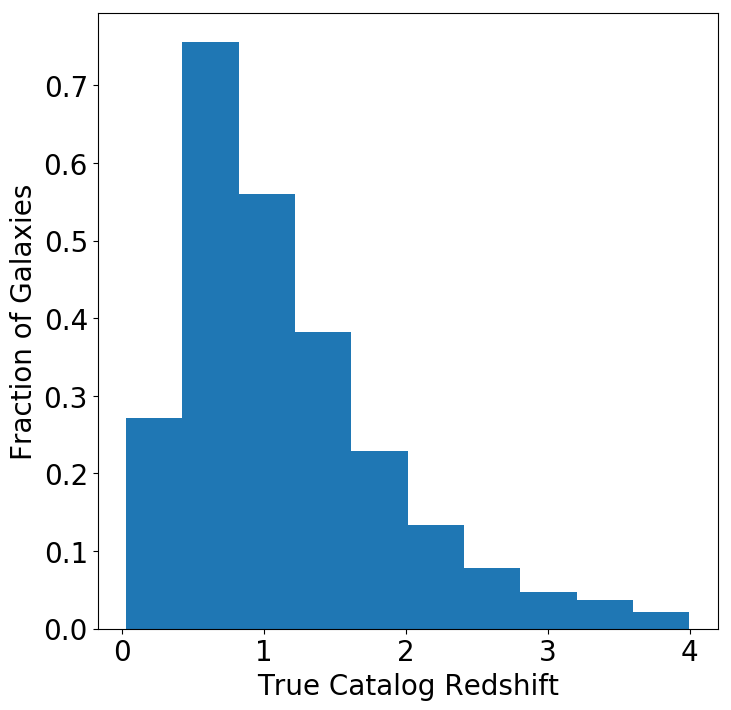
\includegraphics[width=1.\textwidth]{../plots/figure_true_redshift_histogram.png}



\section{Experimental Results}




\section{Analysis of Results and Discussion}



\section{Conclusion}
In \cite{gpz} they use principal component analysis to further pre-process the features, speeds up optimization.


\bibliographystyle{abbrv}
\bibliography{bib.bib}

\end{document}
